% !TEX root = main.tex

\section{Introduction}


\begin{frame}{TODO}
*) LLVM tools other than OPT\\
*) MCA: what it is for (feat. ACA exercise)\\
*) LLVM performance models\\
\end{frame}


\begin{frame}{LLVM Tools}
LLVM provides several \alert{tools} for various purposes:
\medskip
\begin{itemize}
\item Working with LLVM-IR modules
	\begin{itemize}
	\item \texttt{llvm-as}, \texttt{llvm-dis}, \texttt{opt}, \texttt{llc}, \texttt{lli}, \texttt{llvm-link}
	\end{itemize}
\item GNU binutils replacements
	\begin{itemize}
	\item \texttt{llvm-addr2line}, \texttt{llvm-ar}, \texttt{llvm-cxxfilt}, \texttt{llvm-objcopy}
	\item \texttt{llvm-objdump}, \texttt{llvm-ranlib}, \texttt{llvm-readelf}
	\item \texttt{llvm-size}, \texttt{llvm-strings}, \texttt{llvm-strip}
	\end{itemize}
\item LLVM-Developer-specific tools
	\begin{itemize}
	\item \texttt{FileCheck}, \texttt{tblgen}, \texttt{lit}, \texttt{llvm-build}
	\item \texttt{llvm-exegesis}, \texttt{llvm-pdbutil}, \texttt{llvm-locstats}
	\end{itemize}
\item \ldots
\pause
\textbf{
\item Performance analysis
	\begin{itemize}
	\item \texttt{llvm-mca}
	\end{itemize}
}
\end{itemize}
\end{frame}


\begin{frame}{LLVM-MCA}
\texttt{llvm-mca} is a \alert{performance analysis tool}\\
\begin{itemize}
\item It uses information available in LLVM (e.g. scheduling models)
\item Evaluates statically the performance of machine code in a specific CPU.
\end{itemize}

\bigskip
Performance is measured in terms of:\\
\begin{itemize}
\item throughput
\item processor resource consumption
\end{itemize}

\bigskip
The tool currently works for processors with an out-of-order backend for which there is a scheduling model available in LLVM.
\end{frame}


\begin{frame}{Throughput?}
\begin{center}
\emph{
Throughput is defined as\\\textbf{the total amount of work done in a given time}.\cite{hennessy2011computer}\\
}

\bigskip
Translated in terms of \emph{machine code instructions}:\\
\bigskip

\emph{
Throughput is defined as\\\textbf{the total number of instructions executed in a given time}.\\
}

\bigskip
According to this definition,\\the measurement unit of throughput is the \alert{MIPS}\\(Mega-Instructions Per Second)\\
\medskip
\footnotesize{Incidentally (or not...) this is also the name of a CPU architecture!}
\end{center}
\end{frame}


\begin{frame}{Throughput?}{Throughput and Microarchitecture I}
\begin{center}
{\LARGE However...}\\\Large
\bigskip
In modern processors the machine code instruction is not the fundamental unit of computation anymore!
\end{center}
\end{frame}


\begin{frame}{Throughput?}{Throughput and Microarchitecture I}
In modern processors:
\begin{enumerate}
\item Instructions are usually represented in a \alert{CISC-like} compact encoding
	\begin{itemize}
	\item This is now true even for architectures that have a RISC heritage like ARM
	\item Memory latency $\gg$ decoding latency $\Rightarrow$ Code density $\gg$ Decoding overhead
	\end{itemize}
\item The CISC-like encoding is \emph{transformed on-the-fly} to \alert{microcode instructions}
	\begin{itemize}
	\item Select important instructions correspond directly to single microcode instructions
	\item Implementation of more complex instructions stored as \alert{microcode programs} in an internal ROM
	\item Small amount of on-chip SRAM available for patches (microcode updates)
	\end{itemize}
\end{enumerate}
\end{frame}


\begin{frame}{Throughput?}{Throughput and Microarchitecture II}
In modern processors:
\begin{enumerate}
\setcounter{enumi}{2}
\item The microcode instructions are put in a queue and issued to the functional units
\begin{itemize}
	\item Multiple instructions can be evicted from the queue at the same time
	\item Superscalar architecture: multiple \alert{functional units} can act in parallel to serve the microinstructions
	\item \alert{Reservation stations} (in Intel parlance: \alert{Execution Ports}) are decoupled from the functional units (one station can serve multiple functional units)
	\item Register accesses are handled using \alert{explicit register renaming}
	\end{itemize}
\end{enumerate}
\bigskip
The entire execution pipeline revolves around \alert{microinstructions}
\end{frame}


\begin{frame}{Throughput?}{Throughput and Microarchitecture III}
\begin{center}
In modern processors merely measuring the instructions executed per seconds is \alert{insufficient}!\\
\bigskip
Instead we would like to measure the number of \alert{microinstructions} per second.
\end{center}
\end{frame}


\begin{frame}{Throughput?}{Throughput and Microarchitecture IV}
It's not that easy!
\begin{itemize}
\item The microprocessor does not give any visibility into its microcode
\item Microprocessor manufacturers consider their internal microcode ISA a \alert{key competitive advantage} and won't release any detailed information about it
\end{itemize}
\bigskip
\begin{centering}
$\Downarrow$\\
\end{centering}
\bigskip
Performance analysis of a program is a \alert{imperfect statistical science} based on \alert{approximations} of the behavior of a processor derived from \alert{black-box reverse-engineering}.
\end{frame}


\begin{frame}{Processor Resource Consumption?}{Throughput and Microarchitecture V}
Another key element in performance analysis is that \alert{we cannot derive realistic numbers without a reasonably accurate model of the processor}

\begin{itemize}
\item Latency of each Functional Unit
\item Throughput of each Functional Unit
\item Number and kind of Functional Units
\item Number of Reservation Stations
\item Size of the Internal Register File
\item Number of Pipeline Stages (Issue Width)
\item Microinstruction cache size
\item Number of microinstructions per MC instruction
\end{itemize}

{\footnotesize And there's already a lot to it, even though we are ignoring RAM fetch/store, branch prediction, forwarding...}
\end{frame}


\begin{frame}{Processor Resource Consumption?}{Throughput and Microarchitecture V}
This is why \alert{processor resource consumption} is important!
\bigskip
\begin{itemize}
\item It allows to compute the throughput of a piece of code accurately
\item It gives information on the \alert{margin of improvement} that can be achieved
\end{itemize}
\end{frame}


\begin{frame}{Why LLVM-MCA}
In the past, performance analysis was done:
\begin{itemize}
\item by \alert{experimentation} with a wide variety of test machines and CPUs
\item with \alert{manual analysis} using microarchitectural information
\end{itemize}

\begin{centering}
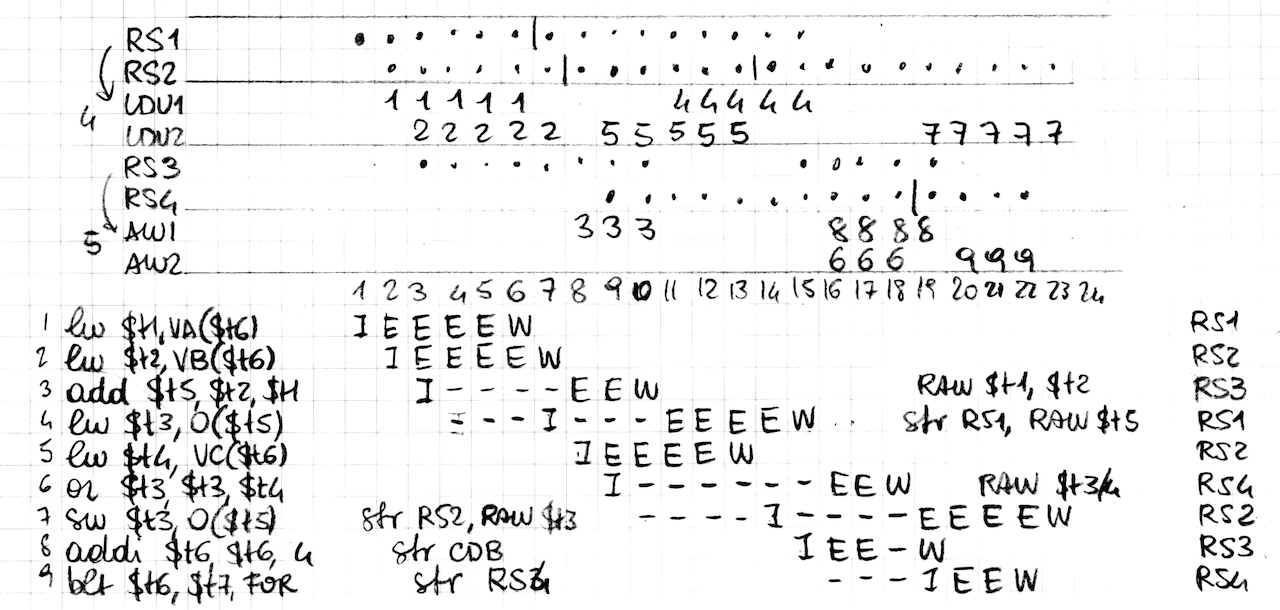
\includegraphics[width=0.9\textwidth]{img/manual-perf-analysis.jpg}\\
\end{centering}
\end{frame}


\begin{frame}{Why LLVM-MCA}
By using an automated tool, we can \alert{improve} the quality of the analysis,
and make it easier to perform.\\
\medskip
\begin{columns}
\column{0.7\textwidth}
\lstinputlisting[basicstyle=\tt\tiny,columns=fullflexible,keepspaces=true]{listings/example-mca-out.txt}
\end{columns}
\end{frame}











